\chapter{密度泛函理论计算方法}\label{chap:dft}

本章讨论一种常用的求解固体电子结构的方法:\concept{密度泛函理论(DFT)}。
直接求解介质中的所有电子在库仑相互作用下的状态是极为困难的,但是我们将看到,原则上总是可以找到一个不依赖于具体系统的泛函,使得任何一个哈密顿量为\eqref{eq:electron-gas-hamiltonian}的系统的任何性质都可以通过最小化这个泛函得到。
这样的计算原则上不需要引入任何经验参数,因此属于\concept{第一性原理计算}。(还有很多其它属于第一性原理计算的方法)
虽然这么说,在实际的第一性原理计算中还是需要一些经验性的东西,如泛函的选取;并且,很多时候难以通过适当选取泛函来捕捉到一些特别近距离而强烈的相互作用(如Hubbard相互作用),从而需要使用所谓的DFT+$U$方法等。
DFT计算如今也经常和Hartree-Fock近似、PRA近似等方法联合使用。

具体来说我们将主要介绍\concept{KSDFT},即基于Kohn-Sham方程的DFT方法,因为它一方面是基于能量泛函的,一方面能够直接给出一些关于单电子波函数的信息。

\section{KSDFT的理论基础与算法}

\subsection{为什么需要密度泛函理论}

DFT的出现让凝聚态体系的无经验参数模拟成为可能。直接求解多体薛定谔方程基本上是不现实的,因为自由度实在太多。
直接求解$10^{23}$量级的电子的波函数本身完全是胡扯;利用周期性条件,求解一个晶胞中的$N$个电子的波函数,则需要求解一个有$3N$个坐标的薛定谔方程,还是非常困难。

在\autoref{sec:ext-e}中我们使用电子数密度标记系统状态并获得了正确的静态结果。一种想法是,有没有可能一般的相互作用电子气的行为也可以完全用它的基态电子数密度来确定。
如果果真如此,我们可以首先将能量表示成电子数密度的泛函,然后最小化这个泛函,就得到了关于该相互作用电子气的一切信息。
电子数密度满足的方程中只有$3$个坐标,这样做,如果可行的话,将大大降低计算量。

\subsection{Hohenberg-Kohn定理}

我们首先说明前述泛函的存在性。本节将通过两个定理,说明的确可以找到一个关于基态电子密度的泛函,使得我们只要最小化这个泛函即可原则上获得关于系统的所有性质。

我们有\concept{Hohenberg-Kohn第一定理}:基态非简并、动能项和相互作用势能项固定、外加势能项是只和位置有关的单粒子算符的哈密顿量\eqref{eq:electron-gas-hamiltonian-sq}的基态电子密度可以唯一确定哈密顿量,即基态电子密度和这类哈密顿量有一一对应的关系。(或者,说得更加明确一些,基态电子密度和\eqref{eq:electron-gas-hamiltonian}中的$V(\vb*{r})$是一一对应的)
其中,电子密度为
\begin{equation}
    \rho(\vb*{r}) = \mel{\Psi}{{\psi}^\dagger(\vb*{r}) {\psi}(\vb*{r})}{\Psi}.
\end{equation}
这个定理的证明如下。如果两个哈密顿量是相同的那么它们当然会给出一样的基态电子密度。
而如果两个哈密顿量不相同却给出了一样的基态电子密度,设这两个哈密顿量是
\[
    {H}_1 = {T} + {V}_\text{int} + {V}_1
\]
和
\[
    {H}_2 = {T} + {V}_\text{int} + {V}_2,
\]
且记每个粒子的外加势能分别是$V_1(\vb*{r})$和$V_2(\vb*{r})$,它们的基态分别是$\ket{\Psi_1}$和$\ket{\Psi_2}$,基态能量为$E_1$和$E_2$,则
\[
    \mel{\Psi_1}{{T} + {V}_1}{\Psi_1} = E_1, \quad \mel{\Psi_2}{{T} + {V}_2}{\Psi_2} = E_2,
\]
且由基态唯一性有
\[
    \mel{\Psi_2}{{T} + {V}_1}{\Psi_2} > E_1, \quad \mel{\Psi_1}{{T} + {V}_2}{\Psi_1} > E_2,
\]
两式相减就得到
\[
    \mel{\Psi_1}{{V}_2 - {V}_1}{\Psi_1} > E_2 - E_1, \quad \mel{\Psi_2}{{V}_1 - {V}_2}{\Psi_2} > E_1 - E_2,
\]
而
\[
    \mel{\Psi}{{V}}{\Psi} = \int \dd[3]{\vb*{r}} \mel{\Psi}{{\psi}^\dagger(\vb*{r}) V(\vb*{r}) {\Psi}(\vb*{r})}{\psi} = \int \dd[3]{\vb*{r}} = \int \dd[3]{\vb*{r}} \rho(\vb*{r}) V(\vb*{r}),
\]
于是上式等价于
\[
    \int \dd[3]{\vb*{r}} \rho_1(\vb*{r}) (V_2(\vb*{r}) - V_1(\vb*{r})) > E_2 - E_1, \quad \int \dd[3]{\vb*{r}} \rho_2(\vb*{r}) (V_1(\vb*{r}) - V_2(\vb*{r})) > E_1 - E_2.
\]
既然$\rho_1(\vb*{r}) = \rho_2(\vb*{r})$,以上两个不等式意味着$0 > 0$,而这当然是不正确的,因此如果基态电子密度一样,那么哈密顿量就不可能不同。
这就证明了Hohenberg-Kohn第一定理。

Hohenberg-Kohn第一定理意味着,只需要基态电子密度就足够确定一个\eqref{eq:electron-gas-hamiltonian-sq}型体系,因为\eqref{eq:electron-gas-hamiltonian}中的动能项都是一样的。
因此这样一个体系的所有性质都可以写成基态电子密度的泛函。
这个看起来不可思议的结论来自电子-原子核体系\eqref{eq:electron-gas-hamiltonian}只是所有可能的体系中的很小一部分这一事实。

实际上,还可以将Hohenberg-Kohn第一定理推广到可能具有简并基态的哈密顿量上。定义\concept{Levy-Lieb泛函}:
\begin{equation}
    \begin{aligned}
        E_\text{LL} [V_\text{ion}(\vb*{r}), \rho(\vb*{r})]  &= \underbrace{\min_{\rho[\psi]=\rho(\vb*{r})} \mel{\psi}{{T} + {V}_\text{int}}{\psi}}_{F_\text{LL}} + \int \dd[3]{\vb*{r}} \rho(\vb*{r}) V_\text{ion} (\vb*{r}) \\
        &= \min_{\rho[\psi]=\rho(\vb*{r})} \mel{\psi}{{T} + {V_\text{int}} + {V}_\text{ion}}{\psi},
    \end{aligned}
    \label{eq:levy-lieb}
\end{equation}
它的取值肯定不会低于系统的基态能量,而如果$\rho(\vb*{r})$正好是外加势$V_\text{ion}(\vb*{r})$对应的电子密度,那么$\ket{\psi}$的取值范围当中肯定包括所有基态,于是$E_\text{LL}$给出了基态能量,而且这是该泛函的极小值。
既然如此,记$\rho_0(\vb*{r})$为$V_\text{ion}(\vb*{r})$对应的电子密度,固定外加势不动对Levy-Lieb泛函做优化,其中$\rho(\vb*{r})$满足约束
\[
    \int \dd[3]{\vb*{r}} \rho(\vb*{r}) = 1,
\]
那么由拉格朗日乘子法,一定有%
\footnote{注意$\lambda$是一个常数而不是一个场,而变分通常都是一个场。}%
\[
    \eval{\fdv{E_\text{LL}}{\rho(\vb*{r})}}_{\rho(\vb*{r}) = \rho_0 (\vb*{r})} = \lambda,
\]
这也就是说
\[
    \eval{\fdv{F_\text{LL}}{\rho(\vb*{r})}}_{\rho(\vb*{r}) = \rho_0(\vb*{r})} + V_\text{ion} = \lambda,
\]
而可以通过别的优化方程计算出$\lambda$,这样实际上我们已经写出了$V_\text{ion}$关于$\rho_0(\vb*{r})$的表达式(可以差一个常数),因此可以从$\rho_0(\vb*{r})$把$V_\text{ion}$恢复出来,也即所有$V_\text{ion}$和所有可能的基态电子密度是一一对应的。
因此Hohenberg-Kohn第一定理对具有简并基态的\eqref{eq:electron-gas-hamiltonian-sq}型系统也使用。
总之,求解出了基态电子密度,我们就获得了一个系统的所有信息,关于这个系统的所有物理量都可以通过基态电子密度的某个泛函计算出来。

一旦有了以上结论,就得到\concept{Hohenberg-Kohn第二定理},也即,基态电子密度是固定了$V_\text{ion}$之后的Levy-Lieb泛函(此时称为\concept{能量泛函})的极小值,可以使用变分原理求出。
这个定理的证明只不过是把上面的论述倒过来使用而已:上面的论述表明给定$\rho_0(\vb*{r})$,通过泛函变分可以计算出$V_\text{ion}$,给定了$V_\text{ion}$通过泛函变分也可以计算出$\rho_0(\vb*{r})$,既然基态电子密度让能量泛函最小。
实际上,记外加势能为$V(\vb*{r})$的能量泛函为$E[\cdots]$,用于求解基态电子密度的变分问题就是
\begin{equation}
    \var \left( E[\rho(\vb*{r})] - \mu \left( \int \dd[3]{\vb*{r}} \rho(\vb*{r}) - N \right) \right) = 0.
    \label{eq:dft-variation-principle}
\end{equation}
这个$\mu$的形式看起来很眼熟,似乎就是化学势。实际上如果近独立电子近似成立,它真的就是零温化学势,即费米能。这一点我们在\autoref{sec:single-electron-in-dft}中可以看到。

\subsection{Kohn-Sham方法}

现在的问题是,给定一个$V_\text{ion}$,怎么写出$E[\rho(\vb*{r})]$?
为了让我们能够写下一个明确的能量泛函,需要引入一些辅助手段。
对一个给定的电子数密度$\rho(\vb*{r})$,构造一个乘积态
\begin{equation}
    \ket{\Psi} = \prod_{i=1}^N {\psi}^\dagger_i \ket{0},
    \label{eq:dft-state}
\end{equation}
使得这个乘积态对应的电子数密度就是$\rho(\vb*{r})$,且它正好是\eqref{eq:levy-lieb}中的让$F_\text{LL}$取最小值的那个$\ket{\Psi}$,或者至少与之非常接近。
如果我们最后需要计算的物理量和$\rho(\vb*{r})$之间的关系是足够平滑的,用拟设\eqref{eq:dft-state}就能够得到很好的结果。
需注意$\ket{\psi}$是乘积态并不意味着密度泛函理论是一个单粒子理论,密度泛函理论并不断言$\ket{\psi}$是系统实际的状态,它只是用来辅助计算的一个数学技巧而已。
这样,就有%
\begin{equation}
    E[\rho(\vb*{r})] = \mel{\Psi}{{H}}{\psi} = \mel{\psi}{{T} + {V}_\text{ion} + {V}_\text{int}}{\Psi}.
\end{equation}
记${\psi}_i^\dagger$产生的单粒子波函数为$\phi(\vb*{r})$,则
\begin{equation}
    \rho(\vb*{r}) = \sum_{i=1}^N \abs{\phi_i(\vb*{r})}^2,
    \label{eq:kohn-sham-density}
\end{equation}
或者,为了避免占据数突变造成计算上的困难,我们可以设
\begin{equation}
    \rho(\vb*{r}) = \sum_i f_i \abs{\phi_i(\vb*{r})}^2,
\end{equation}
其中$f_i$通常就是费米分布函数,总之是一个在费米面以下基本上处处为$1$而在费米面以上(在这里就是$i > N$)基本上处处为$0$的函数;还可以对不同$i$乘以适当的权重。
下面的推导取$f_i$为零温费米分布函数,但一模一样的思路适用于任意的$f_i$。
动能和外加势能都是单体算符,因此以$\ket{\Psi}$为本征态之一。动能项应为
\begin{equation}
    T_\text{s} = \mel{\Psi}{{T}}{\Psi} = - \frac{1}{2m} \sum_i \int \dd[3]{\vb*{r}} \phi_i^*(\vb*{r}) \laplacian \phi_i(\vb*{r}),
\end{equation}
这里下标s表示这个动能项实际上是假定$\ket{\Psi}$是自由理论中的多粒子态而计算出来的;如果$\ket{\Psi}$实际上具有强关联效应,那么用它计算动能就会不对头。
但是,$\ket{\Psi}$和系统实际的波函数也没有什么直接关系,$T_\text{s}$和真实的$\mel*{\Psi}{T}{\Psi}$有差别这件事不会有什么影响,因为反正它们的差最后会在$E_\text{XC}$中得到补偿。
单粒子外加势能项为
\begin{equation}
    V = \mel{\Psi}{{V}_\text{ion}}{\Psi} = \sum_i \int \dd[3]{\vb*{r}} V_{\text{ion}}(\vb*{r}) \phi_i^*(\vb*{r}) \phi_i(\vb*{r}) = \int \dd[3]{\vb*{r}} \rho(\vb*{r}) V_\text{ion}(\vb*{r}),
\end{equation}
而二体的库伦势却会带来很大麻烦。当然,如果采用托马斯-费米近似,则唯一剩下的一项就是Hartree项
\begin{equation}
    \mel{\Psi}{{V}_\text{int}}{\Psi} \approx V_{\text{H}} = \frac{1}{2} \int \dd[3]{\vb*{r}} \int \dd[3]{\vb*{r}'} \frac{e^2 \rho(\vb*{r}) \rho(\vb*{r}')}{\abs{\vb*{r} - \vb*{r}'}},
\end{equation}
但是正如我们在Hartree-Fock近似中看到的那样,会有一个交换能,而且Hartree-Fock近似与真实能量还存在偏差(称为\concept{关联能},这种误差肯定会有因为Hartree-Fock近似是一个平均场理论)。既然$\mel{\psi}{{V}_\text{int}}{\psi}$和上式都是$\rho(\vb*{r})$的泛函,交换能也应该是$\rho(\vb*{r})$的泛函,但我们根本写不出它的解析表达式。
因此实际工作中必须猜测一个\concept{交换-关联能}$E_\text{XC}$,从而写出能量泛函
\begin{equation}
    \begin{aligned}
        E[\rho(\vb*{r})] &= T_\text{s}[\rho(\vb*{r})] + V[\rho(\vb*{r})] + V_H[\rho(\vb*{r})] + E_\text{XC} [\rho(\vb*{r})] \\
        &= - \frac{1}{2m} \sum_i \int \dd[3]{\vb*{r}} \phi_i^*(\vb*{r}) \laplacian \phi_i(\vb*{r})
        + \int \dd[3]{\vb*{r}} \rho(\vb*{r}) V_\text{ion}(\vb*{r}) \\
        &+ \frac{1}{2} \int \dd[3]{\vb*{r}} \int \dd[3]{\vb*{r}'} \frac{e^2 \rho(\vb*{r}) \rho(\vb*{r}')}{\abs{\vb*{r} - \vb*{r}'}} + E_\text{XC} [\rho(\vb*{r})].
    \end{aligned}
    \label{eq:kohn-sham-functional}
\end{equation}
将\eqref{eq:kohn-sham-functional}对$\phi_i^*(\vb*{r})$做优化,即求解
\begin{equation}
    \var \left( E[\rho(\vb*{r})] - \sum_i \epsilon_i \left( \int \dd[3]{\vb*{r}} \phi_i^*(\vb*{r}) \phi_i(\vb*{r}) - 1 \right) \right) = 0,
    \label{eq:dft-variation-principle-shem}
\end{equation}
得到
\begin{equation}
    \left( - \frac{1}{2 m} \laplacian + \int \dd[3]{\vb*{r}'} \frac{\rho(\vb*{r}')}{\abs{\vb*{r} - \vb*{r}'}} + V_\text{ion}(\vb*{r}) + V_\text{XC}(\vb*{r}) \right) \phi_i(\vb*{r}) = \epsilon_i \phi_i(\vb*{r}),
    \label{eq:kohn-sham-eq}
\end{equation}
其中
\begin{equation}
    V_\text{XC}(\vb*{r}) \phi_i(\vb*{r}) = \fdv{E_\text{XC}[\rho(\vb*{r})]}{\phi^*_i(\vb*{r})} = \fdv{E_\text{XC}[\rho(\vb*{r})]}{\rho(\vb*{r})} \phi_i(\vb*{r}).
\end{equation}
\eqref{eq:kohn-sham-eq}是一个有$N$个显含$\rho(\vb*{r})$的方程的方程组,称为\concept{Kohn-Sham方程}。
它们与\eqref{eq:kohn-sham-density}联立就给出了所有的$\psi_i(\vb*{r})$,并立即可以求出$\rho(\vb*{r})$,从而完全解出了系统的一切性质。
基本上数值求解\eqref{eq:kohn-sham-eq}的过程可以概括为\autoref{alg:basic-kohn-sham}。

\begin{algorithm}

    \DontPrintSemicolon
    \SetAlgoLined

    \KwData{初始电子密度$\rho_0(\vb*{r})$,容差$\epsilon$,交换关联泛函选取$E_\text{XC}[\rho(\vb*{r})]$}
    \KwResult{Kohn-Sham波函数$\phi_i(\vb*{r})$和对应的本征值$\epsilon_i$}
    
    $i = 1$ \;
    将$\rho_0(\vb*{r})$代入\eqref{eq:kohn-sham-eq}求解得到$\phi_n^{(1)}$和$\epsilon_n^{(1)}$ \;
    将$\phi_n^{(1)}$代入\eqref{eq:kohn-sham-density}计算得到$\rho_1(\vb*{r})$ \;
    \While{$\rho_i(\vb*{r})$和$\rho_{i-1}(\vb*{r})$的差别大于容差$\epsilon$}{
        将$\rho_i$代入\eqref{eq:kohn-sham-eq}求解得到$\phi_n^{(i+1)}$和$\epsilon_n^{(i+1)}$ \;
        $i = i + 1$ \;
    }
    
    \Return{波函数$\phi^{(i)}_n$和本征值$\epsilon^{(i)}_n$}\;

    \caption{Kohn-Sham方程的自洽求解}
    \label{alg:basic-kohn-sham}
\end{algorithm}

我们又一次看到,Kohn-Sham方程的形式基本上就是“一个电荷背景中的单电子”,只不过电子-电子库伦相互作用不仅包括平方反比律(实际上就是Hartree项),还包括一个(形式难以一般地写出的)$V_\text{XC}$,即我们需要求解有效势能
\begin{equation}
    V_\text{eff}(\vb*{r}) = V_\text{ion}(\vb*{r}) + V_\text{XC}(\vb*{r}) + \int \dd[3]{\vb*{r}'} \frac{\rho(\vb*{r}')}{\abs{\vb*{r} - \vb*{r}'}}
\end{equation}
如果近独立电子近似成立,$\epsilon_i$可能就是电子能级。我们将在\autoref{sec:single-electron-in-dft}中看到这一点。
需注意Kohn-Sham方程的解唯一确凿无疑的物理意义就是电荷密度;$\epsilon_i$和$\phi_i$有什么意义是不完全确定的。

Kohn-Sham方程并非做DFT计算的唯一方法。例如,我们可以有Orbital-free DFT,这是一种完全不使用任何波函数的DFT方法,需要写下交换关联泛函$E_\text{XC}$以及一个用电子密度表示动能的泛函,即\concept{动能泛函},然后做最优化。
动能泛函通常比交换关联泛函还要难以写出,因此OFDFT长期以来不受重视,但近年由于找到了一些可靠的动能泛函,OFDFT的高效率让它再次受到量子化学界的关注。

以上算法也可以体现出DFT方法的一个重大缺陷,就是在不和实验对比时很难评估计算精度,也很难系统地提升计算精度。
求解Kohn-Sham方程是一个完全确定性的算法,我们无法使用量子蒙特卡洛中模拟中观察计算结果方差的方法估计本次计算是不是“对头“;另一方面,$E_\text{XC}[\rho(\vb*{r})]$中各项的物理意义不是非常明晰,因此也很难评估如何改进计算精度。

\section{Kohn-Sham方程的建立和求解}

\autoref{alg:basic-kohn-sham}没有给出如下具体内容:如何引入凝聚态系统中原子核的位置、携带的电荷(从而确定材料中的电子总量)等信息,即如何适当地将$V_\text{ion}$和$\mu$引入以列写Kohn-Sham方程;\eqref{eq:kohn-sham-eq}本身是微分方程,它需要做适当的离散化才能被计算机求解,由于它是本征值问题,我们可以将$\phi_i(\vb*{r})$函数在适当的基底(量子化学中通常称为\concept{基组})下展开,这样只需要求解矩阵的本征值问题。

对一个一般的凝聚态系统,\eqref{eq:kohn-sham-eq}中涉及的单电子波函数的个数要和系统中电子的数目($10^{23}$量级)一样多,否则$\rho(\vb*{r})$的总量不正确。
介质中的电子数目是非常多的,从而直接求解\eqref{eq:kohn-sham-eq}并不现实。
然而晶体有周期性结构,这就大大简化了计算,因为只需要计算一个晶胞内的情况即可。
实际上,由于大部分情况下相互作用衰减得很快,我们完全可以假定液体等也有周期性边界条件,只不过此时的晶胞要取得非常大。
于是以下我们将DFT计算中被认为是周期性的单元称为\concept{超胞(supercell)},对固体通常要求超胞取最简单的形式,即原胞,对单分子、液体或是有杂质的系统等则需要取一个较大的超胞。
对杂质,超胞应该包括杂质周围足够大的体态。
对单分子,当超胞足够大时第一布里渊区足够小,从而计算出的所谓“能带”实际上和单独的一个个能级毫无区别。
我们需要指定超胞的几何形状,并且在超胞内给出各个原子核的位置。

凝聚态研究中,由于系统的离散平移对称性,\eqref{eq:kohn-sham-eq}此时也具有离散平移对称性,它的解——也就是$\phi_i(\vb*{r})$——可以看成某个以我们设定的超胞为原胞的晶体中的单电子波函数,从而Bloch定理\eqref{eq:bloch-wavefunction}成立,且$\phi_i(\vb*{r})$中的$i$应该替换成Bloch波矢$\vb*{k}$,能带编号$n$和自旋$\sigma$。(同样,到这里,所谓“能带编号”也未必对应着实际的系统中的能带电子的能带编号;如何诠释它还是不确定的)

\subsection{基于赝势和平面波的Kohn-Sham方程求解}\label{sec:supercell-pwdft}

\subsubsection{平面波基组和赝势}

求解$\phi_{n \vb*{k}}(\vb*{r})$就是要求解$u_{n \vb*{k}}(\vb*{r})$。
由于\eqref{eq:bloch-wavefunction}中的$u(\vb*{r})$具有周期性,它可以被展开成用倒格矢标记的一系列傅里叶分量,因此我们有(为书写方便暂时略去自旋指标)
\begin{equation}
    \phi_{n \vb*{k}}(\vb*{r}) = \frac{1}{\sqrt{V_\text{u.c.}}} \sum_{\vb*{G}} c_{n, \vb*{k}, \vb*{G}} \ee^{\ii (\vb*{k} + \vb*{G}) \cdot \vb*{r}},
\end{equation}
或者,考虑到$\vb*{k}$局限在第一布里渊区中而$\vb*{G}$是倒格矢,从$\vb*{k} + \vb*{G}$可以唯一确定$\vb*{k}$和$\vb*{G}$,有
\begin{equation}
    \phi_{n \vb*{k}}(\vb*{r}) = \frac{1}{\sqrt{V_\text{u.c.}}} \sum_{\vb*{G}} c_{n, \vb*{k} + \vb*{G}} \ee^{\ii (\vb*{k} + \vb*{G}) \cdot \vb*{r}}.
    \label{eq:dft-plane-wave}
\end{equation}
这种选取$\phi_i$的方法称为\concept{平面波DFT(PWDFT)}。
用平面波做基底的好处在于,首先,对自由电子气模型适用的体系它有直接的物理意义,其次,将波函数展开为平面波有成熟的快速傅里叶变换算法,这样效率很高。
这样做也有坏处,首先是只能处理晶格系统(否则需要不可数无限多个平面波),单分子必须放在一个比较大的晶格中才能够正确计算;其次,对高度局域的电子态以及原子核附近波函数的剧烈振荡,需要大量平面波,效率低下,这点可以部分通过赝势解决。

除了平面波以外还有很多常用的基底,比如高斯波包。
以高斯波包为基底是可以不需要任何赝势的,它能够更加精确高效地处理低轨道电子,从而相较于PWDFT能够更好地处理过渡金属等。

\eqref{eq:dft-plane-wave}中的$\vb*{G}$分量在\eqref{eq:kohn-sham-eq}的动能项部分为$(\vb*{k} + \vb*{G})^2 / 2m$,由于实际能够存储的傅里叶分量的个数是有限的,通常会引入一个\concept{截断能},对每个$\vb*{k}$,我们只保留对动能的贡献小于截断能的那些$\vb*{G}$。
这意味着我们忽略了空间尺度特别小的现象,并且忽略了一部分能量,但是如果对应的$c_{n, \vb*{k} + \vb*{G}}$不大就没有什么问题。

实际能够处理的晶体都是有限大小的,或者说实际的$\vb*{k}$的取值是第一布里渊区中离散的一些点。
这就是说,我们需要给出一种“第一布里渊区中的动量采样”。
显然,采样越密越好;可以使用$\vb*{k} \cdot \vb*{p}$来简化计算。

最后我们处理至今尚未提及的$V_\text{ion}$。如\autoref{sec:pseudopotential}所述,外层电子感受到的势场可以用赝势取代。
这里我们有好几种可能的做法:可以只计算外层电子,完全不计算内层电子,从而自始至终$V_\text{ion}$都是用赝势组合而成的,此时截断能可以设置得比较小,因为$\phi_{n \vb*{k}}(\vb*{r})$在靠近原子核的位置也不会发生剧烈振荡;原则上也可以将$V_\text{ion}$取成不同位置的原子的原子核的库伦势场的叠加,这相当于将材料中的所有电子都做了计算,即做了\concept{全电子计算},当然,这样在原子核附近会有非常剧烈的波函数变化,并且高度局域的内层电子都会出现,从而截断能必须取得非常高,基本上是不现实的。
一般来说用不到全电子计算,因为化学反应的能级不足以激发内层电子,倒是从头计算赝势时需要全电子计算。
做全电子计算另有它法,如\autoref{sec:dft-paw},实际上,这给出了系统性地生成赝势的一种方法。
赝势类型本身也非常多样,详细情况见\autoref{sec:dft-pseudo-pot}。
我们也可以将平面波方法称为赝势方法,既然直接用它做全电子计算并不现实。

综上,PWDFT计算需要的输入信息有:
\begin{itemize}
    \item 晶体结构,这包括超胞以及各个原子在超胞内部的位置以及各个原子的类型;
    \item 赝势信息,实际上等于是在描述各个原子都是什么原子;
    \item 第一布里渊区采样,即\eqref{eq:dft-plane-wave}中$\vb*{k}$的密集程度;
    \item 和材料的结构、原子、$\vb*{k}$点采样都无关的东西,如截断能、泛函选取等。
\end{itemize}

\subsubsection{不考虑自旋的PWDFT算法}

\begin{algorithm}

    \DontPrintSemicolon
    \SetAlgoLined

    \KwData{初始电子密度$\rho_0(\vb*{r})$,交换关联泛函选取$E_\text{XC}[\rho(\vb*{r})]$,不同原子的赝势,原胞结构,$\vb*{k}$点采样$K = \{\vb*{k}\}$,原胞中电子总数$N_\text{e}$,截断能$E_\text{cut}$,最大迭代次数$N_\text{max}$,所考虑的最大能带数目$n_\text{max}$,容差$\epsilon$}
    \KwResult{Kohn-Sham波函数$\phi_{n \vb*{k}}(\vb*{r})$和对应的本征值$\epsilon_{n \vb*{k}}$,迭代次数$i$}
    
    \For{$\vb*{k} \in K$}{
        根据$\frac{(\vb*{k} + \vb*{G})^2}{2m} < E_\text{cut}$确定需要考虑的$\vb*{G}$的取值范围$G$ \;
    } 

    $i = 1$ \;
    使用不同原子的赝势和原胞结构构造$V_\text{ion}(\vb*{r})$,并按照\eqref{eq:momentum-space-potential-dft}做傅里叶变换 \;
    使用$\rho_0(\vb*{r})$计算$V_\text{H}$和$V_\text{XC}$,并按照\eqref{eq:momentum-space-potential-dft}做傅里叶变换 \;
    将$V_\text{ion}, V_\text{H}, V_\text{XC}$代入\eqref{eq:kohn-sham-eq-pw-minimal}求解,对每个$\vb*{k}$求前$n_\text{max}$个解,得到$\{c_{n, \vb*{k} + \vb*{G}}^{(1)}\}$和$\{\epsilon_{n, \vb*{k} + \vb*{G}}^{(1)}\}$ \;
    将$\{c_{n, \vb*{k} + \vb*{G}}^{(1)}\}$代入\eqref{eq:pw-minimal-expand}计算出$\{\phi_{n, \vb*{k} + \vb*{G}}^{(1)}\}$ \;
    将$\{\phi_{n, \vb*{k} + \vb*{G}}^{(1)}\}$代入\eqref{eq:kohn-sham-density-pw-minimal}计算得到$\rho_1(\vb*{r})$ \;
    \While{$\rho_i(\vb*{r})$和$\rho_{i-1}(\vb*{r})$的差别大于容差$\epsilon$且$i < N_\text{max}$}{
        使用$\rho_i(\vb*{r})$计算$V_\text{H}$和$V_\text{XC}$,并按照\eqref{eq:momentum-space-potential-dft}做傅里叶变换 \;
        将$V_\text{ion}, V_\text{H}, V_\text{XC}$代入\eqref{eq:kohn-sham-eq-pw-minimal}求解,对每个$\vb*{k}$求前$n_\text{max}$个解,得到$\{c_{n, \vb*{k} + \vb*{G}}^{(i+1)}\}$和$\{\epsilon_{n, \vb*{k} + \vb*{G}}^{(i+1)}\}$ \;
        将$\{c_{n, \vb*{k} + \vb*{G}}^{(i+1)}\}$代入\eqref{eq:pw-minimal-expand}计算出$\{\phi_{n, \vb*{k} + \vb*{G}}^{(i+1)}\}$ \;
        将$\{\phi_{n, \vb*{k} + \vb*{G}}^{(i+1)}\}$代入\eqref{eq:kohn-sham-density-pw-minimal}计算得到$\rho_{i+1}(\vb*{r})$ \;
        $i = i + 1$ \;
    }
    
    \Return{$i$,波函数$\{\phi^{(i)}_{n, \vb*{k} + \vb*{G}}\}$和本征值$\{\epsilon^{(i)}_{n, \vb*{k} + \vb*{G}}\}$}\;

    \caption{给定晶格和原子赝势,不考虑自旋的PWDFT静态自洽计算}
    \label{alg:static-pwdft-minimal}
\end{algorithm}

我们现在可以给出完整的平面波计算的方程和步骤了。首先考虑一个没有必要考虑自旋极化的系统,此时只需要求解轨道部分即可。
以下我们给出一个最简单的PWDFT算法,不考虑$f$,则电子数密度为
\begin{equation}
    \rho(\vb*{r}) = 2 \sum_{n, \vb*{k} \text{ occupied}}  \phi_{n \vb*{k}}(\vb*{r}),
    \label{eq:kohn-sham-density-pw-minimal}
\end{equation}
而$\phi_{n \vb*{k}}$展开为
\begin{equation}
    \phi_{n \vb*{k}}(\vb*{r}) = \frac{1}{\sqrt{V_\text{u.c.}}} \sum_{(\vb*{k} + \vb*{G}) / 2m \leq E_\text{cut}} c_{n, \vb*{k} + \vb*{G}} \ee^{\ii (\vb*{k} + \vb*{G}) \cdot \vb*{r}},
    \label{eq:pw-minimal-expand}
\end{equation}
在此平面波基组下,Kohn-Sham方程是
\begin{equation}
    \begin{aligned}
        &\quad \sum_{( \vb*{k} + \vb*{G}') / 2m \leq E_\text{cut} } \left( \frac{(\vb*{k} + \vb*{G}') ^2}{2m} \delta_{\vb*{G} \vb*{G}'} + V_\text{ion}(\vb*{G} - \vb*{G}') + V_\text{H}(\vb*{G} - \vb*{G}') + V_\text{XC}(\vb*{G} - \vb*{G}') \right) c_{n, \vb*{k} + \vb*{G}'} \\
        &= \epsilon_{n, \vb*{k} + \vb*{G}} c_{n, \vb*{k} + \vb*{G}},
    \end{aligned}
    \label{eq:kohn-sham-eq-pw-minimal}
\end{equation}
其中动量空间的势能由
\begin{equation}
    V_\text{ion}(\vb*{r}) = \frac{1}{\sqrt{V_\text{u.c.}}} \sum_{\vb*{G}} V(\vb*{G}) \ee^{\ii \vb*{G} \cdot \vb*{r}}
    \label{eq:momentum-space-potential-dft}
\end{equation}
定义,$V_\text{H}(\vb*{G})$和$V_\text{XC}(\vb*{G})$类同。
将以上细节填充进\autoref{alg:basic-kohn-sham}中,我们得到\autoref{alg:static-pwdft-minimal},即所谓\concept{静态自洽计算}。(说是“静态”是因为有时候我们对晶体结构只有一个大概的猜测,此时需要做结构优化,即所谓\concept{结构优化自洽计算},这个是要变动晶体结构的,而静态自洽计算不变动晶体结构)
只要输入的晶体信息是准确的,交换关联泛函的质量足够好,我们就得到了外层电子的模拟结果。

可以看到,虽然DFT没有任何经验参数,并且将每一条可能的能带都纳入考虑,截断能、$\vb*{k}$点采样、赝势的选择、泛函的选择会显著影响计算精度,对它们的选择是需要一些经验的;我们的确不需要根据实验数据拟合一些经验参数输入计算程序,但是很多时候是需要根据实验事实决定选择哪个赝势、哪个泛函的。

\autoref{alg:static-pwdft-minimal}有不少可以扩充的地方。
在实际的DFT软件包中,通常不会将各次迭代的波函数和本征值留到计算结束再输出,而是在每次循环中把计算结果写入一个输出文件中,这样如果某一步计算失败了,已经写入的数据还可以用;也可以不以$\rho_0(\vb*{r})$为初始值而是以一组波函数为初始值。

\subsection{全电子计算的APW方法和LAPW方法}\label{sec:dft-lapw}

% TODO:也可以用赝势计算出初步的电子密度,然后改用库伦势做进一步计算?

\subsection{PAW方法}\label{sec:dft-paw}

如前所述,使用平面波方法计算全电子问题有现实中难以克服的困难,即需要非常多的平面波来模拟原子核附近的电子行为。


\begin{info}{VASP软件包}{vasp}
    VASP是维也纳大学维护的一个商业DFT包,基于平面波和各种缀加平面波。其输入文件有四个,正好对应四种输入:
    \begin{itemize}
        \item \texttt{POSCAR},给出一个平行六面体超胞的三个初基格矢,以及各个原子的类型、数目,用笛卡尔坐标系或是晶体坐标系给出的坐标。
        \item \texttt{POTCAR},赝势文件。
        \item \texttt{KPOINTS},动量采样,有多种方案。
        \item \texttt{INCAR},计算中的参数,截断能、泛函选择、最大计算步数、能带数目、容差等。
    \end{itemize}
\end{info}

\section{泛函选择}

本节讨论如何构造和选择合适的交换关联泛函$E_\text{XC}[\rho(\vb*{r})]$;在DFT的语境下,交换关联泛函经常就简称“泛函”。
库仑定律的形式告诉我们,交换关联泛函的形式肯定是不局域的,因为有$\abs{\vb*{r} - \vb*{r}'}$这样的因子,并且同时要对$\vb*{r}$和$\vb*{r}'$两个变量求积分。
但实际上由于屏蔽作用等这种空间上的非局域性衰减得很快,于是密度关联泛函总是可以写成以下的局域表达式:%
\footnote{
    如果非局域性衰减得很快,那么可以做多级展开
    \[
        f(\vb*{r} - \vb*{r}') = f(\vb*{r}) + (\vb*{r} - \vb*{r}') \cdot \grad{f} + \cdots,
    \]
    这样就可以先积掉$\vb*{r}'$这个变量,得到
    \[
        \int \dd[3]{\vb*{r}} \dd[3]{\vb*{r}'} f(\vb*{r} - \vb*{r}') = \int \dd[3]{\vb*{r}} g(f(\vb*{r}), \grad{f(\vb*{r})}, \ldots).
    \]
}%
\[
    E_\text{XC}[\rho(\vb*{r})] = \int \dd[3]{\vb*{r}} f(\rho(\vb*{r}), \grad{\rho(\vb*{r})}, \ldots),
\]
而由于交换能与$\rho(\vb*{r})$的平方同阶,通常会设
\begin{equation}
    E_\text{XC}[\rho(\vb*{r})] = \int \dd[3]{\vb*{r}} \rho(\vb*{r}) \epsilon_\text{XC}(\rho(\vb*{r}), \grad{\rho(\vb*{r})}, \ldots).
\end{equation}

常用的交换-关联泛函的形式包括以下几种:
\begin{itemize}
    \item \concept{局域密度近似(LDA)}:$\epsilon_\text{XC}[\rho(\vb*{r})] = \epsilon_\text{XC}(\rho(\vb*{r}))$;
    \item \concept{广义梯度近似(GGA)}:$\epsilon_\text{XC}[\rho(\vb*{r})] = \epsilon_\text{XC}(\rho(\vb*{r}), \grad{\rho(\vb*{r})})$;
    \item \concept{Meta-GGA}:在GGA近似中加入一个动能密度修正(基本上是$\laplacian \rho(\vb*{r})$);
    \item \concept{混合泛函}:Hartree-Fock近似和别的一些东西的线性组合;
    \item \concept{经验泛函}:有一大堆参数,根据实际数据微调参数。
\end{itemize}
不同泛函的分类如\autoref{fig:excahnge-correlation-functional}所示。

\begin{figure}
    \centering
    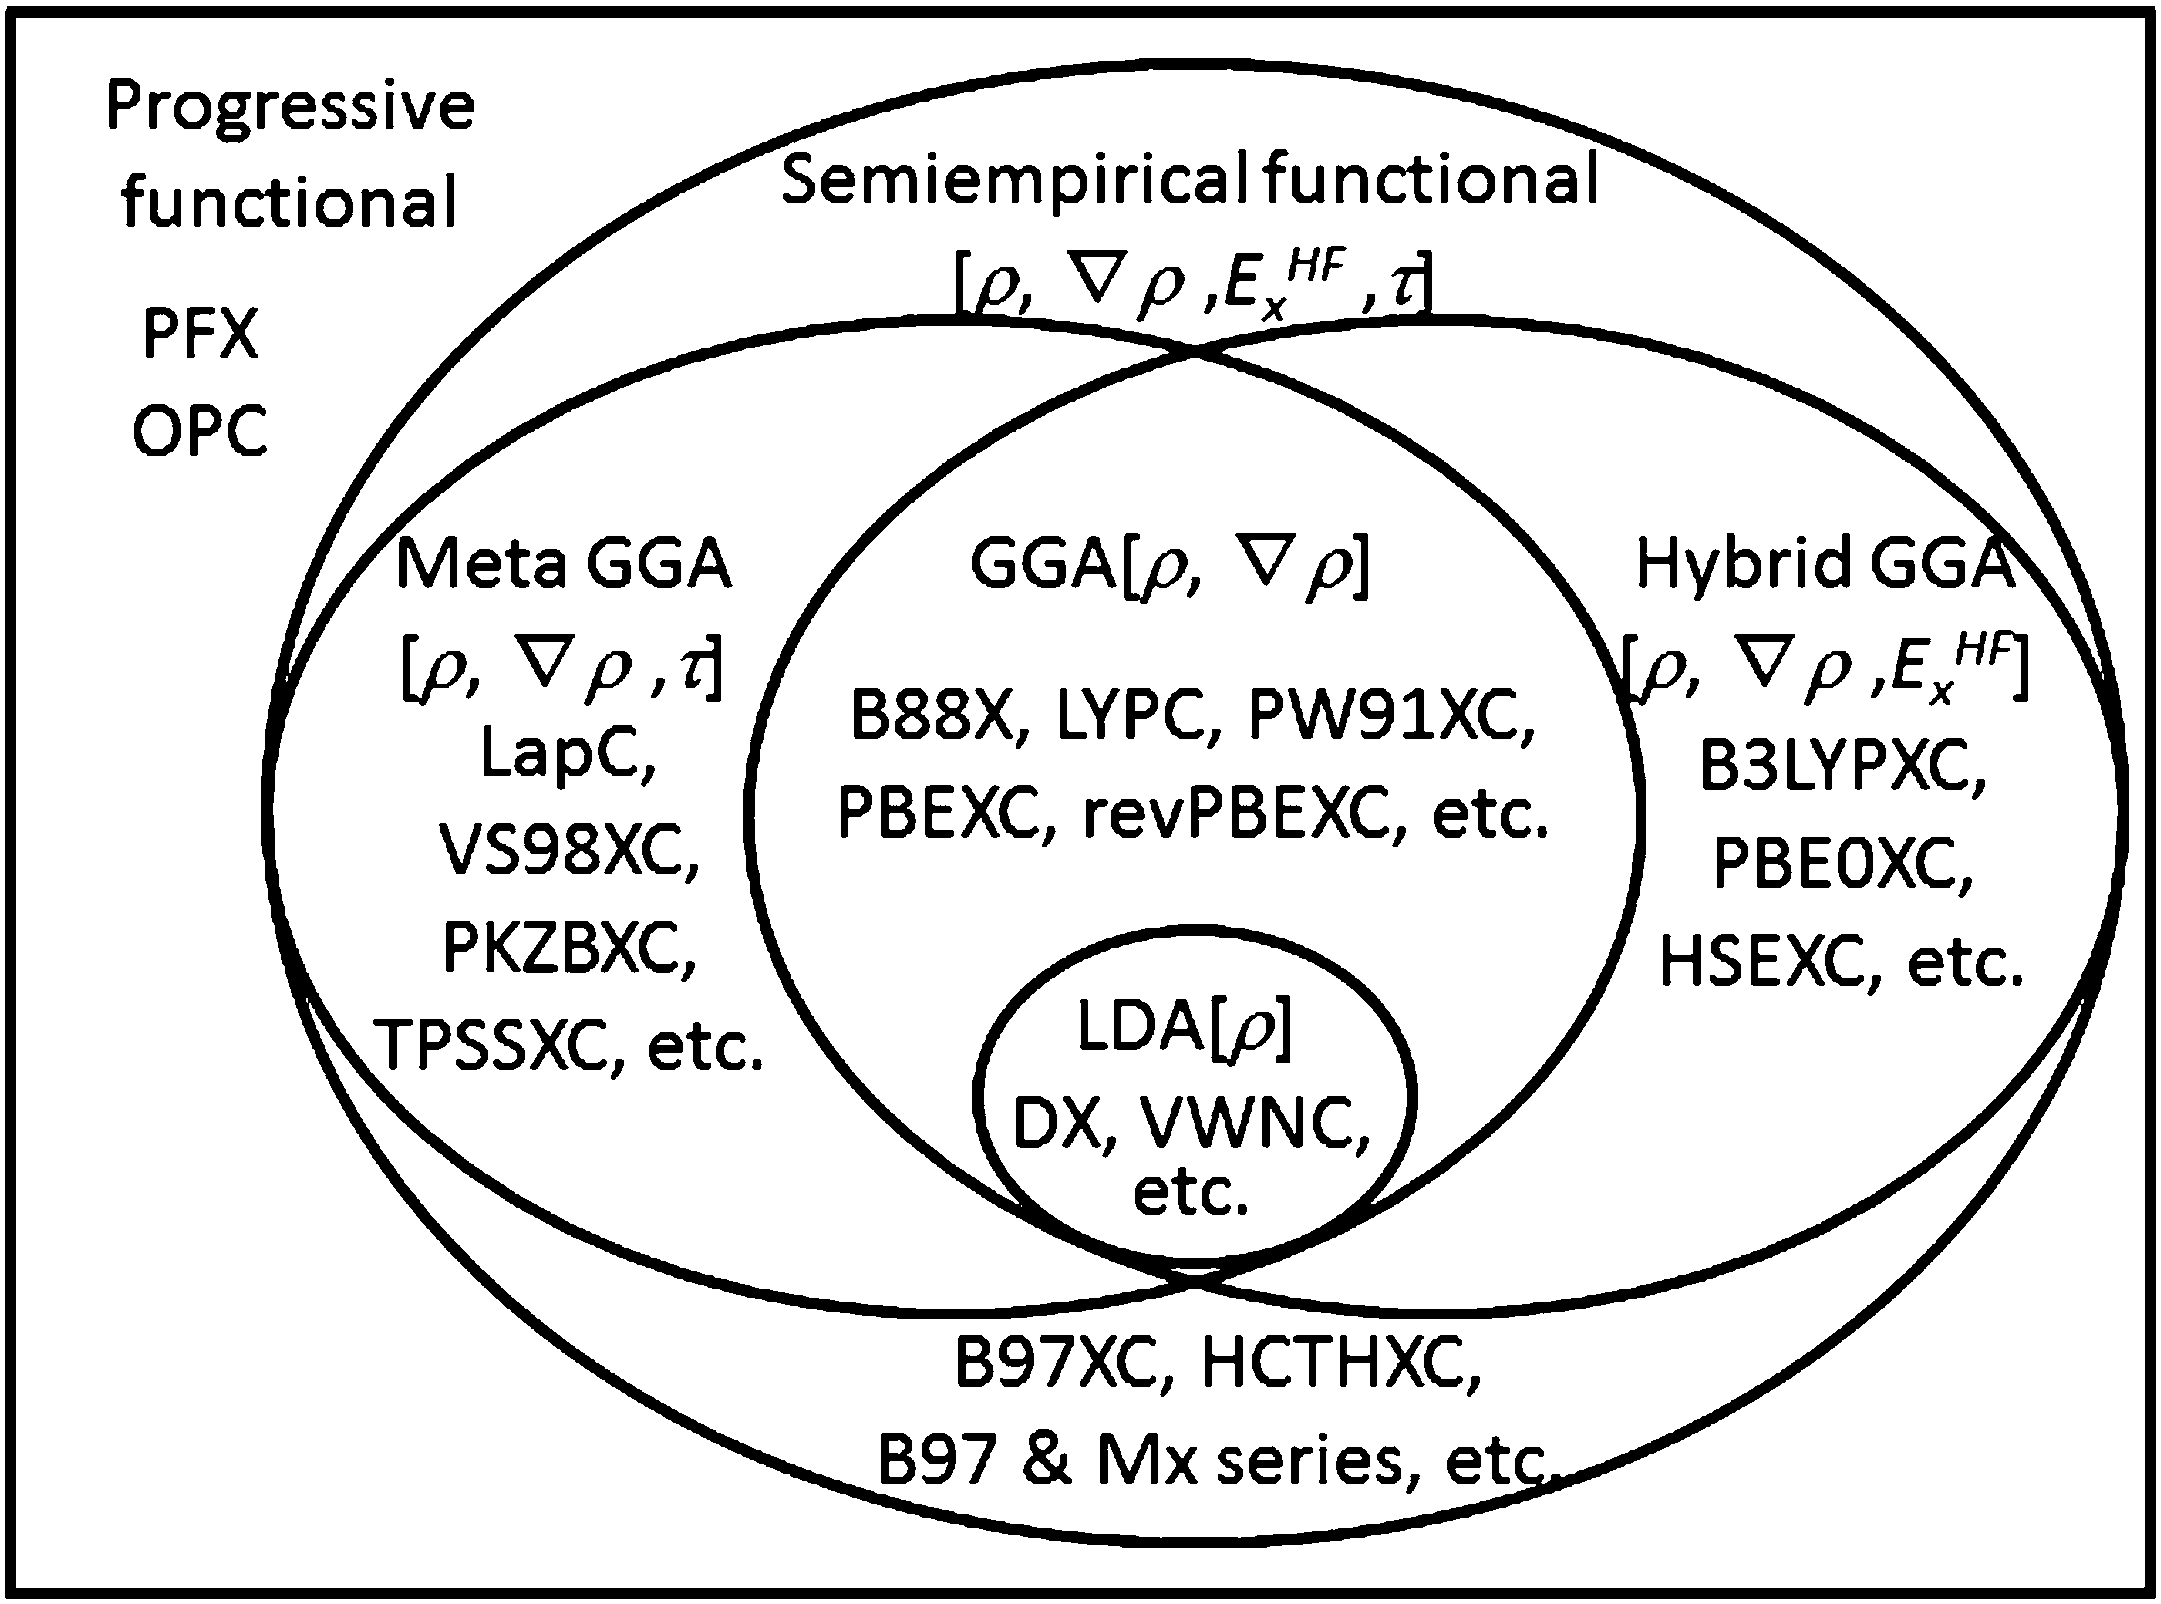
\includegraphics[width=0.5\textwidth]{functional-classification.png}
    \caption{交换-关联泛函的分类}
    \label{fig:excahnge-correlation-functional}
\end{figure}

目前并没有能够准确计算一切体系的$E_\text{XC}$,没有也是很正常的,因为很明显,这个泛函需要的复杂程度和“看着库仑相互作用想出一切可能的凝聚态现象”是一样的,后者不可能做到,前者当然不可能做到。
但是对特定的体系,一些相互作用通道可以忽略,一些误差可以互相抵消,找到一个复杂程度适中的泛函描述它们是可以做到的。
适当地构造和选择泛函非常需要技术含量和经验。

最后,虽然原则上一切库仑相互作用导致的物理效应都可以通过$E_\text{XC}[\rho(\vb*{r})]$得到,这件事实际上做起来并不那么容易。
如果一个泛函被证明能够模拟一些相互作用通道导致的物理而无法模拟另一些,我们就需要手动向一个没有可调参数的$E_\text{XC}[\rho(\vb*{r})]$引入一些修正项。
这些修正项的大小往往无法固定下来,因为不同情况下$E_\text{XC}[\rho(\vb*{r})]$对对应的相互作用通道的忽略可能也是不一样的。
手动引入Hubbard排斥(所谓LDA+$U$,涉及非常短程的相互作用,不容易被比较光滑的泛函模拟)、范德瓦尔斯力(长程,不容易被比较局域的泛函模拟)就是例子。

\subsection{LDA近似}

当电子密度变化非常平缓时,$\grad{\rho},\laplacian{\rho}$等全部可以看成是零,此时交换关联泛函的形式是
\begin{equation}
    E_\text{XC}[\rho(\vb*{r})] = \int \dd[3]{\vb*{r}} \rho(\vb*{r}) \epsilon_\text{XC}(\rho(\vb*{r})).
\end{equation}
这就是所谓的\concept{局域密度近似(LDA)}:每单位的交换关联能只和该地点的电子密度有关。

我们主要将尝试寻找一个适用于均匀电子气的交换关联泛函。均匀电子气指的是没有晶格、也没有外场时的库伦相互作用电子气,其电荷密度是处处均匀的。
由于无论是均匀电子气还是电子密度较平缓但是的确有晶格周期势的电子气理论上均共享一种$E_\text{XC}$,而对它们LDA近似均适用,如果我们找到了一个$E_\text{XC}[\rho(\vb*{r})]$可以精确地预言均匀电子气的行为,那么这个泛函也应该能够比较精确地预言一般的、电子密度较平缓的电子气的行为。

\subsubsection{Hartree-Fock近似和托马斯-费米-狄拉克泛函}

自由电子气的基态就是费米面以内的每个轨道都占据了一上一下两个电子的状态,我们设共有$N$个电子,那么这些电子占据了$N/2$个不同的轨道。设这些轨道为$\{\phi_i(\vb*{r})\}$。
仅考虑库伦相互作用引入的一阶微扰,则有
\[
    E = \sum_{\sigma, \sigma'} \mel{\Psi}{
        \frac{1}{2} \int \dd[3]{\vb*{r}} \dd[3]{\vb*{r}'} {\psi}^\dagger_{\sigma}(\vb*{r}) {\psi}^\dagger_{\sigma'}(\vb*{r}') \frac{e^2}{\abs{\vb*{r} - \vb*{r}'}} {\psi}_{\sigma'}(\vb*{r}') {\psi}_\sigma(\vb*{r})
    }{\Psi}.
\]
这里必须完整地考虑自旋自由度的作用。可以使用Wick定理把上式展开,这就是在做Hartree-Fock近似。
请注意由于均匀电子气中没有自旋翻转,任何形如
\[
    \mel{\Psi}{{\psi}_\sigma^\dagger {\psi}_{\sigma'}}{\Psi}, \quad \sigma \neq \sigma'
\]
的项都是零,而
\[
    \mel{\Psi}{{\psi}^\dagger_\sigma(\vb*{r}) {\psi}_{\sigma}(\vb*{r}')}{\Psi} = \sum_i \phi_i^*(\vb*{r}) \phi_i(\vb*{r}'),
\]
于是最后能量修正为
\[
    E = \frac{1}{2} \int \dd[3]{\vb*{r}} \dd[3]{\vb*{r}'} \frac{e^2}{\abs{\vb*{r} - \vb*{r}'}} \bigg(
        \underbrace{4 \sum_{i} \abs{\phi_i(\vb*{r})}^2 \sum_{i} \abs{\phi_i(\vb*{r}')}^2}_\text{classical coulomb energy, Hartree term} - \underbrace{2 \sum_i \phi_i^*(\vb*{r}) \phi_i(\vb*{r}') \sum_i \phi_i^*(\vb*{r}') \phi_i(\vb*{r})}_\text{exchange energy}
    \bigg).
\]
交换能项前面的因子是$2$而不是$4$是因为自旋不同的电子之间的交换能全部抵消了。这样交换能就是
\begin{equation}
    E_\text{X} = - \int \dd[3]{\vb*{r}} \dd[3]{\vb*{r}'} \frac{e^2}{\abs{\vb*{r} - \vb*{r}'}} \abs{\sum_i \phi_i^*(\vb*{r}) \phi_i(\vb*{r}')}^2 . 
    \label{eq:exchange-energy-homogeneous-gas}
\end{equation}
对箱归一化的均匀电子气,有
\[
    \phi_i(\vb*{r}) = \frac{1}{\sqrt{V}} \ee^{- \ii \vb*{k}_i \cdot \vb*{r}},
\]
于是就有
\begin{equation}
    \sum_i \phi_i^*(\vb*{r}) \phi_i(\vb*{r}') = \sum_{\text{occupied $\vb*{k}$}} \frac{1}{V} \ee^{\ii \vb*{k} \cdot (\vb*{r} - \vb*{r}')} = \frac{1}{(2\pi)^3} \int_{\abs{\vb*{k}} < k_\text{F}} \dd[3]{\vb*{k}} \ee^{\ii \vb*{k} \cdot (\vb*{r} - \vb*{r}')},
    \label{eq:homogeneous-density}
\end{equation}
特别的,电子密度的一半(因为只考虑了轨道自由度)为
\[
    n(\vb*{r}) / 2 = \frac{k_\text{F}^3}{6 \pi^2}.
\]
上式代入\eqref{eq:exchange-energy-homogeneous-gas}就得到交换能的形式。
在这里我们稍微做一些推广。考虑一个非均匀的自由电子气,其非均匀性可能来自一些杂质或者特殊的相互作用,总之,每一个宏观小微观大的体积元可以看成一个用于归一化波函数的箱子,波函数定域在这个箱子里面(杂质会导致局域化)。
这样只有$\vb*{r} - \vb*{r}'$不超出一个箱子时\eqref{eq:homogeneous-density}才有明显的非零值。
每个箱子都有自己的费米动量,记作$k_\text{F}(\vb*{r})$(具体是关于$\vb*{r}$还是$\vb*{r}'$无关紧要因为两者总是在同一个箱子内)。
令
\[
    \vb*{s} = \vb*{r} - \vb*{r}', 
\]
则
\[
    \begin{aligned}
        E_\text{X} &= - e^2 \int \dd[3]{\vb*{r}} \dd[3]{\vb*{s}} \frac{1}{s} \left( \frac{1}{(2\pi)^3} \int_{\abs{\vb*{k}} < k_\text{F}} \dd[3]{\vb*{k}} \ee^{\ii \vb*{k} \cdot \vb*{s}} \right)^2 \\
        &= - e^2 \int \dd[3]{\vb*{r}} \dd[3]{\vb*{s}} \frac{1}{s} \left( \frac{3}{2} \frac{\sin t - t \cos t}{t^3} n(\vb*{r}) \right)^2 \quad (t= k_\text{F}(\vb*{r}) s) \\
        &= - 9 e^2 \pi \int \dd[3]{\vb*{r}} \int \dd{t} \frac{t}{k_\text{F}(\vb*{r})^2} n(\vb*{r})^2 \left( \frac{\sin t - t \cos t}{t^3} \right)^2 \\
        &= - e^2 \frac{3}{4} \left( \frac{3}{\pi} \right)^{1/3} \int \dd[3]{\vb*{r}} \rho(\vb*{r})^{4/3}.
    \end{aligned}
\]
这就得到了\concept{托马斯-费米-狄拉克泛函}:
\begin{equation}
    E_\text{X}[\rho(\vb*{r})] / e^2 = - \frac{3}{4} \left( \frac{3}{\pi} \right)^{1/3} \int \dd[3]{\vb*{r}} \rho(\vb*{r})^{4/3} = - 0.7386 \int \dd[3]{\vb*{r}} \rho(\vb*{r})^{4/3}.
    \label{eq:thomas-fermi-dirac-functional}
\end{equation}
对均匀或不均匀但缓变的电子气这个泛函确定适用。

对一般的系统,托马斯-费米-狄拉克泛函当然是不那么精确的,但是我们可以以它为更精确的泛函的起点。
\eqref{eq:thomas-fermi-dirac-functional}本质上是Hartree-Fock近似中的Fock项,那么要修正它,加入关联能就可以,即我们需要尝试寻找一个$E_\text{C}$使得
\begin{equation}
    E_\text{XC}[\rho(\vb*{r})] = E_\text{X}[\rho(\vb*{r})] + E_\text{C}[\rho(\vb*{r})].
\end{equation}
这个$E_\text{C}$就称为\concept{关联泛函}。

\subsubsection{关联泛函的量子蒙特卡洛计算}

关联泛函就是正确的$E_\text{XC}$减去\eqref{eq:thomas-fermi-dirac-functional}。

\subsection{GGA近似}

从LDA近似的推导中可以清楚地看到,一旦离开了均匀电子气模型,LDA近似的可靠性就不好说了。
对那些电子密度确定会有比较大的空间起伏的系统——比如说在我们需要精确计算分子结构时——LDA近似的精度不是特别好,此时有必要引入GGA近似。

\subsection{杂化泛函:将Hartree-Fock近似结合进DFT}

\subsection{LDA+$U$}

\subsection{范德瓦尔斯力}

\section{赝势}\label{sec:dft-pseudo-pot}

本节讨论赝势如何生成。\autoref{sec:pseudopotential}中的做法不考虑任何电子-电子相互作用而计算内层电子的轨道,即把介质中的原子当成类氢原子,但是这样无疑精度非常糟糕。
不过做DFT计算实际上就是求解\eqref{eq:kohn-sham-eq-pw-minimal},这形式上仍然是一个单电子方程,因此“计算波函数,然后把高频振荡抹平”的做法仍然是适用的。

\section{物理量测量和后处理}

本节讨论Kohn-Sham方程求解完成后怎样从计算结果解读出我们需要的各个物理量,在第一性原理计算的语境下也可以称为“非自洽计算”,因为就是拿到了电荷密度,然后算各种东西,无需迭代求解Kohn-Sham方程。
这件事是没那么容易的,基本上和基态电子密度有解析形式关系的量就是基态能量,基态能量实际上就是能量泛函作用在基态电子密度$\rho(\vb*{r})$之后的结果。
除此以外的东西——比如第一激发态能量——和Kohn-Sham方程求解结果之间都没有特别平凡的关系。

% TODO:类似于确定每一条带上的电子磁矩如何,电荷密度等等

\subsection{单电子诠释和能带}\label{sec:single-electron-in-dft}

\subsubsection{Kohn-Sham方程的解的物理意义}

在待计算的系统确实适用单电子诠释时,我们将\eqref{eq:kohn-sham-eq}和\eqref{eq:dyson-wave-eq}对比,很容易看出两者的相似之处。
如果Hartree项加上$V_\text{XC}$构成对自能$\Sigma$的一个良好模拟,那么\eqref{eq:kohn-sham-eq}解出的$\epsilon_i$\emph{就是}能带电子的能量。

如果实际情况确实如此,那么\eqref{eq:dft-variation-principle}中的$\mu$实际上就是费米能,因为对比\eqref{eq:dft-variation-principle}和\eqref{eq:dft-variation-principle-shem}会发现
\begin{equation}
    \mu = \sum_{i=1}^N \epsilon_i.
\end{equation}

\subsubsection{GW计算}

GW计算实际上是一种独立的数值计算方法,但是因为它要求一个比较接近实际情况的单电子波函数作为起点,我们仍然可以将它视为DFT的后处理的一部分,即将DFT计算出来的Kohn-Sham波函数作为GW计算的初始值。

\subsection{原子受力}

在计算单原子受力时我们最好把晶胞扩张得大一些。如果使用原胞做计算,那么将某个原子移动一小段得同时,其它原胞中与它地位一致的原子也发生了移动,因此通过这种方式计算原子移动前后的能量变化并进一步计算力是不准确的。
相反,如果晶胞被扩张了,那么移动一个原子之后,与之最为接近的那些原胞中与之地位一致的原子并没有发生移动,会给出相对可靠的结果。

有时候我们对晶体结构只有一个大概的猜测,此时需要做结构优化,即所谓\concept{结构优化自洽计算}。